\section{Background}

\subsection{Nonlinear Correctors}

To compensate for errors locally, both sides of the LHC IRs hosting experiments 
(ATLAS in IR1, ALICE in IR2, CMS in IR5 and LHCb in IR8) are equipped with linear and non-linear corrector packages.
As shown in the schematics of \cref{fig:irregionlhc,fig:irregionhllhc}, 
these packages are located within the common aperture region of the machines, between Q3 and the separation dipoles D1,
and hence contain common magnets for the two beams. 
Any correction should therefore take the optics of both beams into account.

In the experimental IRs of the LHC and in HL-LHC IR2 and IR8, nonlinear correctors for
skew and normal sextupoles ($a_3, b_3$), skew and normal octupoles ($a_4, b_4$) 
and normal dodecapoles ($b_6$) are available.
In IR1 and IR5 in the HL-LHC on the other hand, the corrector package will be upgraded to 
also include skew and normal decapoles ($a_5, b_5$) as well as skew dodecapoles ($a_6$)
and offer therefore a wider range of field errors to correct, to account for the 
increase in the $\beta$-function in this high-performance 
machine~\cite{AberleHighLuminosityLargeHadron2020,DeMariaHighLuminosityLHC2019,BuffatOpticsMeasurementCorrection2022}.


Some correctors were defective in LHC Run~2 and Run~3:
\ttt{MCSSX.3L2, MCOX.3L2, MCOSX.3L2}, the skew sextupole, octupole and skew ocupole correctors left of IP2, possibly due to a hit from a pilot beam,
as well as \ttt{MCOSX.3L1}, the skew octupole corrector left of IP1, probably due to powering issues. 
This is already reflected in the lattice used for simulations \cite{DeMariaCERNOpticsRepository}.
% MCSSX.3L2:MCSSX_UNPLUGGED,   
% MCOX.3L2:MCOX_UNPLUGGED,     
% MCOSX.3L2:MCOSX_UNPLUGGED,   
% MCOSX.3L1:MCOSX_UNPLUGGED,   


\begin{figure}[h!]
    \centering
    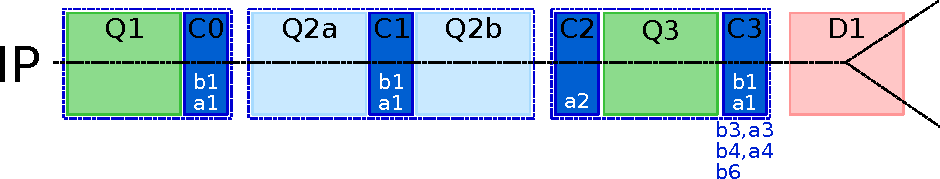
\includegraphics[height=2.5cm]{ir_lhc.pdf}
    \caption{Schematic of the right hand side of a LHC IR region and HL-LHC IR2 and IR8.
    Q1, Q2a/b and Q3 are the triplet quadrupoles.
    C0-C3 show the corrector packages with the field order to be corrected indicated. 
    Blue lines mark common cryostats. 
    D1 is the separation dipole, diverging Beam~1 and Beam~2
    to their respective beamlines. 
    The non-linear corrector package is included with the orbit correctors in C3.
    }
    \label{fig:irregionlhc}
\end{figure}


\begin{figure}[h!]
    \centering
    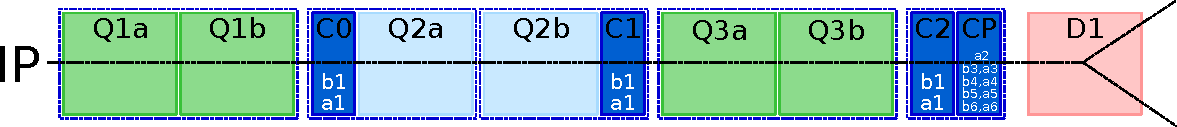
\includegraphics[width=\textwidth]{ir_hllhc.pdf}
    \caption{Schematic of the right hand side of HL-LHC IR1 and IR5.
    Q1a/b, Q2a/b and Q3a/b are the triplet quadrupoles. 
    C0-C2 and CP show the corrector packages with the field order to be corrected indicated. 
    D1 is the separation dipole, diverging Beam~1 and Beam~2
    to their respective beamlines. 
    Blue lines mark common cryostats. 
    }
    \label{fig:irregionhllhc}
\end{figure}


\subsection{Resonance Driving Terms}

The transformation of the phase-space coordinates of a particle propagating through an accelerator 
from $s'$ to $s$ can be described by means of maps $\mathcal{M}(s', s)$, 
each describing the transformation of the coordinates generated by the elements of the machine between the locations.
These maps are symplectic, i.e. they preserve phase-space volume, and can be combined, describing the propagation 
through multiple elements of the accelerator~\cite{DragtLieSeriesInvariant1976}.
Using the In a circular accelerator one can construct a one-turn-map $\mathcal{M}_\circ $, 
describing the coordinate transformation of one complete turn. 
For an ideal accelerator consisting of purely \textit{linear} elements, 
one can use the Courant-Snyder formalism~\cite{CourantTheoryAlternatinggradientSynchrotron1958} 
to express the coordinates of the phase-space
as a vector $\bm{c} = (c_{x,+}, c_{x,-}, c_{y,+}, c_{y,-})$ of complex coordinates in action $J_z$ (the invariant of linear motion) and phase $\phi_z$
%
\begin{equation}
    \label{eq:CSCoordinates}
    c_{z,\pm} = \hat{z} \pm i\hat{p}_z = \sqrt{2J_z}e^{\mp i \phi_z} \, ,
\end{equation}
%
for $z \in \{x, y\}$, where $\hat{z}$ and $\hat{p}_z$ are the canonical position and momentum, 
related to the cartesian position $z$ and momentum $p_z$ via the $\alpha$- and 
$\beta$-functions at any location $s$ by 
%
\begin{equation}
    \begin{pmatrix}\hat{z}(s) \\ \hat{p}_z(s) \end{pmatrix} = 
    \begin{pmatrix} \sfrac{1}{\sqrt{\beta_z}(s)} & 0 \\ \sfrac{\alpha_z(s)}{\sqrt{\beta_z(s)}} & \sqrt{\beta_z(s)}\end{pmatrix}
    \begin{pmatrix}z(s) \\ p_z(s)\end{pmatrix}
    \;.
\end{equation}

With \cref{eq:CSCoordinates} propagation through the accelerator is described by rotations, 
e.g. to a longitudinal location $s$ by advancing the phase from $s_0$ to $s$ by 
%
\begin{equation}
    \label{eq:PhaseAdvance}
    \Delta\phi_z(s_0, s) = \phi_z(s) - \phi_z(s_0) = \int\limits_{s_0}^s \frac{1}{\beta(s')} \mathrm{d}s' \, 
\end{equation}
%
meaning the coordinates at $s$ of a particle can be given as the initial coordinates at $s_0$ propagated to $s$
%
\begin{equation}
    \label{eq:CSCoordinatesAtLocation}
    c_{z,\pm}(s) = \hat{z}(s) \pm i\hat{p}_z(s) = \sqrt{2J_z}e^{\mp i \phi_z(s) } = \sqrt{2J_z}e^{\mp i \left(\phi_{z,0} + \Delta\phi(s_0, s)  \right)}  = \mathcal{M}_{z,\pm}(s_0, s) \cdot c_{z,\pm}(s_0)\, ,
\end{equation}
where $\phi_{z,0} = \phi_z(s_0)$ is the initial phase of the particle, $J_z = J_z(s) \equiv J_z(s_0)$ its action
and $\mathcal{M}_{z,\pm}$ are the components of $\mathcal{M} = (\mathcal{M}_{x,+}, \mathcal{M}_{x,-},\mathcal{M}_{y,+},\mathcal{M}_{y,-})$ propagating $\bm{c}$.
%
In this linear system, the linear one-turn-map of an accelerator of circumference $C$ is then also a rotation $\mathcal{M}_\circ = R$
by $\Delta\phi_z(s, s+C) = 2\pi Q_z$, where $Q_z$ are the \textit{tunes} of the accelerator:
\begin{equation}
    \label{eq:PropagationOfC}
    c_{z,\pm}(s + C) = \mathcal{M}_{z,\pm,\circ} \cdot c_{z,\pm}(s) = e^{\mp i2\pi Q_z} c_{z,\pm}(s)  = \sqrt{2J_z}e^{\mp i \left(\phi(s) + 2\pi Q_z\right) }
\end{equation}

In \cite{BengtssonAnalyticalCalculationsSmear1990,ForestHamiltonianFreeDescription1990,TomasDirectMeasurementResonance2003,FranchiStudiesMeasurementsLinear2006,CarlierNonlinearFutureMeasurements2020}
this formalism is extended to derive a transformation, such that the propagation also through a \textit{nonlinear} circular machine, 
i.e. a circular accelerator containing additional nonlinear elements, 
can be described by an amplitude dependent rotation and is shortly summarized here.


Using Lie-Algebra notation~\cite{DragtLieSeriesInvariant1976, DragtLieAlgebraicTheory1982} we can define an operator $:\cdot:$ as
%
\begin{equation}
    \label{eq:LieOperator}
    :g: = \sum\limits_{z=x,y} \frac{\partial g}{\partial q_z} \frac{\partial }{\partial p_z} - \frac{\partial g}{\partial p_z} \frac{\partial }{\partial q_z} \;,
\end{equation}
%
for a function $g(q_x, p_x, q_y, p_y)$ of canonical coordinates, e.g. positions/momenta $\left( x, p_x, y, p_y \right)$ or actions/angles $\left( J_x, \phi_x, J_y, \phi_y\right)$.
It is shown that the, now location dependent, nonlinear one-turn map can be expressed as
\begin{equation}
    \label{eq:OTMNormalized}
    \mathcal{M}_\circ(s) = e^{:h(s):}R  \; ,
\end{equation}
%
where $R$ is still a rotation containing the linear contributions of the system and $h(s)$
is an integral of the Hamiltonians $H_w$ of the nonlinear elements $w$ of the accelerator,
expressed as functions of powers of the normalized coordinates $c_{z, \pm}(s_w)$, 
but these coordinates propagated (linearly) backward from the origin $s_w$ of the nonlinear sources to $s$.
Or, maybe more intuitively, the particle at $s$ is being propagated linearly through the ring, 
experiencing the influence of the nonlinearities at their locations. 

If the nonlinearities $H_w$ in the machine are small
$h(s)$ can be approximated, truncating the Baker-Campbell-Hausdorff formula at first order of $H_w$  
%
\begin{equation}
    \label{eq:hamiltonianTwissCoordinates}
    \newcommand{\rint}{\oint\limits_{\text{Ring}}}
    \newcommand{\ds}{\,\mathrm{d}s}
    \begin{split}
    &h(s) \approx   \rint H_w(s_w, s) \ds_w =\\
    &\sum\limits_{jklm} \; \rint
     h_{jklm}(s_w) 
    e^{i\left[(j-k)\Delta \phi_x(s, s_w) + (l-m)\Delta \phi_{y}(s, s_w)\right]} c_{x,+}^j(s_w)  c_{x,-}^k(s_w)  c_{y,+}^l(s_w)  c_{y,-}^m(s_w) \ds_w 
    % = \\
    % &\sum\limits_{jklm} \; \rint
    % h_{jklm}(s_w) \; (2J_x)^{\frac{j+k}{2}}(2J_y)^{\frac{l+m}{2}} 
    % e^{-i\left[(j-k)(\phi_x(s_w) + \Delta \phi_x(s_w, s)) + (l-m)(\phi_y(s_w) + \Delta \phi_{y}(s_w, s))\right]} \ds_w 
    % =\\ 
    % &\sum\limits_{jklm} \; \rint
    % h_{jklm}(s_w)  \ds_w \; 
    % (2J_x)^{\frac{j+k}{2}}(2J_y)^{\frac{l+m}{2}} 
    % e^{-i\left[(j-k)\phi_x(s)  + (l-m)\phi_y(s)\right]}
    % =\\  
    % &\sum\limits_{jklm} \; \rint
    % h_{jklm}(s_w)  \ds_w \; 
    % c_{x,+}^j(s)  c_{x,-}^k(s)  c_{y,+}^l(s)  c_{y,-}^m(s) 
    \; .
    \end{split}
\end{equation}
%
The sum $jklm$ is over all possible values of $j,k,l$ and $m$ and
$h_{jklm}$ are parts of the in $\bm{c}$ expanded Hamiltonians of all sources of multipole order 
$n = j + k + l + m$ (see \cite{FranchiStudiesMeasurementsLinear2006}~Appendix~A).
The contribution $h_{jklm}$ from magnetic fields of order $n \geq 2$ to the total Hamiltionian of the system is given 
e.g. in \cite{FranchiStudiesMeasurementsLinear2006} Eq.~(3.11) as 
%
\begin{equation}
    \label{eq:HamiltonianTermsMultipoleSources}
    h_{jklm}(s) = 
    -\ReOf{    
     \frac{i^{l+m}}{j! \, k! \, l! \, m! \, 2^{j+k+l+m}}
    \beta_x(s)^{\frac{j+k}{2}}\beta_y(s)^{\frac{l+m}{2}} 
    \left(K_{n}(s) + iJ_{n}(s)\right)
     } \; .
\end{equation}
%
$K_n(s)$ and $J_n(s)$ are the magnetic field strengths of order $n$ at location $s$ of normal and skew fields respectively.
In this note, we use the convention of starting the index $n$ at $1$, representing dipole fields 
($n=2$ for quadrupole fields, etc.).

It has been neglected up until now that, with nonlinearities present in the machine,
the the phase-space is distorted and $J_z$ is no longer the invariant of motion.
Similar to \cref{eq:CSCoordinates}, a new coordinate vector $\bm{\zeta}$ can be found, 
depending on new action and angle coordinates $I_z$ and $\psi_z$
%
\begin{equation}
    \label{eq:NFCoordinates}
    \zeta_{z,\pm} = \sqrt{2I_z}e^{\mp i \psi_z} \, ,
\end{equation}
%
called normal form,
in which the one-turn map $\mathcal{M}_I$ can again be split into a nonlinear part 
and a the same rotation $R$ as in \cref{eq:OTMNormalized}
%
\begin{equation}
    \label{eq:OTMNormalizedI}
    \mathcal{M}_I = e^{:h_I:}R  \; ,
\end{equation}
%
now with the Hamiltonian series $h_I$ only dependent on $I_z$, making $M_I$ independent of location.
A variable transformation can be constructed,
translating between $\bm{c}$ and $\bm{\zeta}$, 
to make use of the simplicity of \cref{eq:OTMNormalizedI}:
\begin{equation}
    \label{eq:NormalFormTransformation}
    \mathcal{M}_\circ(s) = e^{:F(s):} \;  \mathcal{M}_I \; e^{:-F(s):} \; .
\end{equation}
%
$F(s)$ is calculated as 
%
\begin{equation}
    \label{eq:NormalFormGeneratingFunction}
    % Going with the sign-convention of Rogelio's Thesis 3.31 here
    F(s) = \sum\limits_{jklm} f_{jklm}(s)  \zeta_{x,+}^j(s) \zeta_{x,-}^k(s)  \zeta_{y,+}^l(s)  \zeta_{y,-}^m(s) 
    %  = \sum\limits_{jklm} f_{jklm}(s) (2I_x)^{\frac{j+k}{2}}(2I_y)^{\frac{l+m}{2}} e^{-i\left[(j-k)\psi_x(s) + (l-m)\psi_y(s)\right]} 
    \; .
\end{equation}
% 
The generating terms $f_{jklm}$ of $F$ are the so called Resonance Driving Terms (RDTs) and it is shown 
in~\cite{ForestHamiltonianFreeDescription1990} (also given in \cite{FranchiStudiesMeasurementsLinear2006} Eq. (3.15)) 
that their relation to the $h_{jklm}(s)$ in \cref{eq:hamiltonianTwissCoordinates} is
%
\begin{equation}
    \label{eq:RDTHamiltonianRelation}
    f_{jklm}(s) = 
    \frac{h^{\oint}_{jklm}(s)}{1 - e^{i2\pi[(j-k)Q_x + (l-m)Q_y]}}  = 
    \frac{ 
    \oint_\text{Ring} h_{jklm}(s_w) 
    e^{i\left[(j-k)\Delta \phi_x(s, s_w) + (l-m)\Delta \phi_{y}(s, s_w)\right]} \mathrm{d}s_w
    }{1 - e^{i2\pi[(j-k)Q_x + (l-m)Q_y]}}
    \;.
\end{equation}
%
Sometimes the numerator $h^{\oint}_{jklm}(s)$ of \cref{eq:RDTHamiltonianRelation} is already called RDT.
In case of the condition 
%
\begin{equation}
    \label{eq:ResonanceCondition}
    (j-k) \cdot Q_x + (l-m) \cdot Q_y = 2\pi \cdot p 
\end{equation}
%
being fulfilled for $p \in \mathbb{Z}$, $f_{jklm}$ diverges, if there are sources present for that order.
In this case the system is in a resonant state, and hence unstable.
The behaviour of the instability as the system approaches the resonance condition therefore depends 
on the strength of the multipole sources present in the machine.
Resonances labeled ($n_x$, $n_y$) are driven by all $h_{jklm}$ terms such that $n_x = j-k$ and $n_y = l - m$.

For each resonance ($n_x$, $n_y$) there is a  spectral component in the turn-by-turn particle position data,
which can be found at $-(n_x-1) \cdot Q_x - n_y \cdot Q_y$ (label: $(-n_x+1, -n_y)$) in the spectrum of the horizontal plane 
and $-n_x \cdot Q_x - (n_y - 1) \cdot Q_y$ (label: $(-n_x, -n_y+1)$) in the spectrum of the vertical plane~\cite{FranchiStudiesMeasurementsLinear2006}.
The amplitude of the spectral lines is proportional to $\left| f_{jklm} (s) \right|$~\cite{FranchiStudiesMeasurementsLinear2006},
the terms are therefore easily accessible from measurements~\cite{SchmidtMeasurementDrivingTerms2001,TomasDirectMeasurementResonance2003,TomasMeasurementGlobalLocal2005,FranchiFirstSimultaneousMeasurement2014,CarlierObservationsResonanceDriving2016}.

As long as there are no sources of order $n$, $|f_{jklm}(s)|$ are constant along $s$.
At the location of a multipole source, the value of $|f_{jklm}(s)|$ changes, 
making them very well suited to build local observables~\cite{TomasMeasurementGlobalLocal2005}.
The correction algorithm presented here is based on locally minimizing the RDTs in the IR as shown in the next section. 

\subsection{Correction Principle}
\label{sec:CorrectionPrinciple}
 
In this section the correction principle as implemented in
the flexible correction algorithm v1.0.0 in~\cite{OMC-TeamIRNLRDTCorrection} is described.
The algorithm follows the simplifications of \cref{eq:HamiltonianTermsMultipoleSources,eq:RDTHamiltonianRelation} 
as outlined in~\cite{BruningDynamicApertureStudies2004}:

\begin{mytemize}
    \item Only the contribution from elements in one IR to the RDTs are minimized.
          The integral in \cref{eq:RDTHamiltonianRelation} includes therefore only IR elements.
    \item Constant coefficients of \cref{eq:RDTHamiltonianRelation} are ignored, 
          i.e. the numerator and actions as well as the coefficients depending only on $j,k,l,m$ and any signs,
          as they are not needed for minimization, .
    \item The phase of one side of the IR is approximately constant, as $\beta(s)$ being very large in the triplets
          and therefore the integral \cref{eq:PhaseAdvance} very small. 
    \item The phase-advance between the left and right side of the IP is $\pi$. 
    \item The RDT is evaluated locally at the entrance of the IR. 
\end{mytemize}

With these approximations \cref{eq:RDTHamiltonianRelation} 
becomes a local, \textit{effective} RDT to minimize within the IR:
%
\begin{equation}
    \label{eq:effectiveRDT}
    f^\text{IR}_{jklm} =  \int\limits_\text{IR} 
    \ReOf{    
     i^{l+m}
     \left(K_{n}(s) + iJ_{n}(s) \right) 
    }
        \beta_x(s)^{\frac{j+k}{2}}
        \beta_y(s)^{\frac{l+m}{2}} 
     e^{i \pi n \theta(s - s_\text{IP})}
    \mathrm{d}s \; ,
\end{equation}
%
with $\theta(x)$ being the Heaviside step function and $s_\text{IP}$ the location of 
the IP within the IR.
The exponential function should actually contain $j - k + l - m = n - 2k - 2l$, 
which is even when $n$ is even and odd when $n$ is odd. 
As $e^{i\pi} = -1$, only the parity of the exponent is important, 
independent of the particular choices for $j,k,l,m$,
and hence $n$ is used for simplicity.

The main concept of the correction is then to find the $K_n(s)$ and $J_n(s)$ of 
the corrector magnets, that minimize a set of given $f^\text{IR}_{jklm}$ based on given optics.

As there are usually two correctors per multipole field available (one on each side of the IP), 
two combinations of $l+m$ and $j+k$ (the exponents of the $\beta$ function)
can be corrected.
As, due to the single-aperture nature of the magnets close to the IP,
the correctors are responsible for the correction of both beams.
In \cref{sec:DualOptics} it will be explained, how
the $\beta$-exponents can be chosen such that the correction is valid for both beams, 
correcting only a single RDT per beam,
unless the symmetry of the optics can be used to correct two RDTs. 

% In the LHC $a_3, b_3, a_4, b_4$ and $b_6$ correctors are available,
% in the HL-LHC additionally $a_5, b_5$ and $a_6$.


\subsubsection{Equation System}

In our simulations, the input to the correction algorithm will be the output 
of \ttt{TWISS} and \ttt{ESAVE} functions from \ttt{MAD-X}~\cite{CERNMadX}.
These are tables in which $K_n(s)$ and $J_n(s)$ are not continuous functions, 
but given as already integrated values $K_nL_w$, $J_nL_w$ 
(\ttt{K$_{n-1}$L}, \ttt{K$_{n-1}$SL} in the terminology of \ttt{MAD-X}) for each element $w$.
Values for the longitudinal position $s_w$, $\beta_{x,w}, \beta_{x,w}$ and the transversal orbit $x_w, y_w$, which will be important 
when calculating feed-down (see below), are also provided.

One way to get an estimate for the integral in \cref{eq:effectiveRDT}, 
is \textit{slicing} the lattice in \ttt{MAD-X}, 
i.e. approximating the magnets as single kicks surrounded by drift-spaces. 
Long magnets should be cut into multiple of these slices to increase accuracy. 
Corrector magnets on the other hand, which are in any case short compared to e.g. dipoles, 
can  be represented by a single slice.

In this thin-lens approximation, \cref{eq:effectiveRDT} transforms into a sum over all elements (slices) $w$ in the IR, 
which needs to be set (using ``$\overeq{!}$'' to stress the intention) to zero to suppress the RDT:
 %
\begin{equation}
    \label{eq:effectiveRDTSum}
    f^\text{IR}_{jklm} =  \sum\limits_{w \in \text{IR}} 
    \ReOf{    
     i^{l+m}
     \left(K_{n}L_w + iJ_{n}L_w \right) 
    }
        \beta_{x,w}^{\frac{j+k}{2}}
        \beta_{y,w}^{\frac{l+m}{2}} 
     (-1)^{n \theta(s_w - s_\text{IP})} 
     \overeq{!} 0 
     \; .
\end{equation}
%

Splitting the elements into corrector elements $\mathcal{C}$ and non-corrector elements $\text{IR}\setminus\mathcal{C}$,
\cref{eq:effectiveRDTSum} transforms into:
 %
\begin{equation}
    \label{eq:equationSum}
    \begin{split}
    &\;\;\sum\limits_{w \in \mathcal{C}} \;\;
    \ReOf{    
     i^{l+m}
     \left(K_{n}L_w + iJ_{n}L_w \right) 
    }
        \beta_{x,w}^{\frac{j+k}{2}}
        \beta_{y,w}^{\frac{l+m}{2}} 
     (-1)^{n \theta(s_w - s_\text{IP})} \\
     = 
    -&\sum\limits_{w \in \text{IR}\setminus\mathcal{C}} 
    \ReOf{  
     i^{l+m}
     \left(K_{n}L_w + iJ_{n}L_w \right) 
    }
        \beta_{x,w}^{\frac{j+k}{2}}
        \beta_{y,w}^{\frac{l+m}{2}} 
     (-1)^{n \theta(s_w - s_\text{IP})}
     = -I_{jklm}     
     \; ,
    \end{split}
\end{equation}
where $I_{jklm}$ a shorthand for the sum over IR$\setminus\mathcal{C}$.

It is important to note, that each corrector is defined by either
$K_nL$ or $J_nL$, so that per order $n$ and orientation (normal, skew) only a limited set of 
correctors is left.
Normally there are two of these correctors in the LHC/HL-LHC, i.e. one per IP side,
and $\mathcal{C} = \{cl, cr\}$, a left ($cl$) and a right ($cr$) corrector element.
With
\begin{equation}
    \label{eq:BcomponentsDef}
    \begin{split}
    b_{jklm}^{(cl)} &= 
     \hphantom{(-1)^n} \, i^{l+m} \,
     \beta_{x,cl} ^{\frac{j+k}{2}} \beta_{y,cl}^{\frac{l+m}{2}} 
    \\
    b_{jklm}^{(cr)} &= 
     (-1)^n\, i^{l+m} \, 
     \beta_{x,cr} ^{\frac{j+k}{2}} \beta_{y,cl}^{\frac{l+m}{2}} \; ,
    \end{split}
\end{equation}
%
\cref{eq:equationSum} can be split into a two equation system 
%
\begin{equation}
    \label{eq:linearEqSystemSingle}
    \begin{split}
        \begin{pmatrix}
            b_{jklm}^{(cl)} & b_{jklm}^{(cr)}
        \end{pmatrix}
        \begin{pmatrix}
            K_{n}L_{cl} \\ 
            K_{n}L_{cr}
        \end{pmatrix}
        &= - I_{jklm}
        \qquad \text{if } l+m \text{ even},
        \\
        \begin{pmatrix}
            i \, b_{jklm}^{(cl)} & i \, b_{jklm}^{(cr)}
        \end{pmatrix}
        \begin{pmatrix}
            J_{n}L_{cl} \\ 
            J_{n}L_{cr}
        \end{pmatrix}
        &= - I_{jklm}
        \qquad  \text{if } l+m \text{ odd}, 
    \end{split}
\end{equation}
%
each of which can be easily extended to include multiple RDTs, e.g.
with $j+k+l+m = j'+k'+l'+m' = n$ and $l + m \equiv l' + m' \pmod 2$:
\begin{equation}    
    \label{eq:linearEqSystemDouble}
    \begin{split}
        \begin{pmatrix}
            b_{jklm}^{(cl)} & b_{jklm}^{(cr)} \\
            b_{j'k'l'm'}^{(cl)} & b_{j'k'l'm'}^{(cr)}
        \end{pmatrix}
        \begin{pmatrix}
            K_{n}L_{cl} \\ 
            K_{n}L_{cr}
        \end{pmatrix}
        &= - 
        \begin{pmatrix}
            I_{jklm} \\ 
            I_{j'k'l'm'} 
        \end{pmatrix}
        \quad \text{if } l + m \text{ (and } l'+m' \text{) even,} \\
        %
        \begin{pmatrix}
            i \, b_{jklm}^{(cl)}     & i \, b_{jklm}^{(cr)} \\
            i \, b_{j'k'l'm'}^{(cl)} & i \, b_{j'k'l'm'}^{(cr)}
        \end{pmatrix}
        \begin{pmatrix}
            J_{n}L_{cl} \\ 
            J_{n}L_{cr}
        \end{pmatrix}
        &= - 
        \begin{pmatrix}
            I_{jklm} \\ 
            I_{j'k'l'm'} 
        \end{pmatrix}
        \quad \text{if } l + m \text{ (and } l'+m' \text{) odd.}
    \end{split}
\end{equation}
These linear equation systems can be solved or optimized for $K_nL_{cl, cr}$ or $J_nL_{cl, cr}$ by standard algorithms.


\subsubsection{Dual Optics} % --------------------
\label{sec:DualOptics}

% \begin{tikzpicture}
%     \node (start) at (0, 0) {aaa};
%     \node (end) at (1, 1) {bbb};
%     \draw[red, ->]  (start) -- (end);
% \end{tikzpicture}


\begin{figure}[htbp]
    \centering
    \begin{subfigure}[t]{0.35\textwidth}
        % 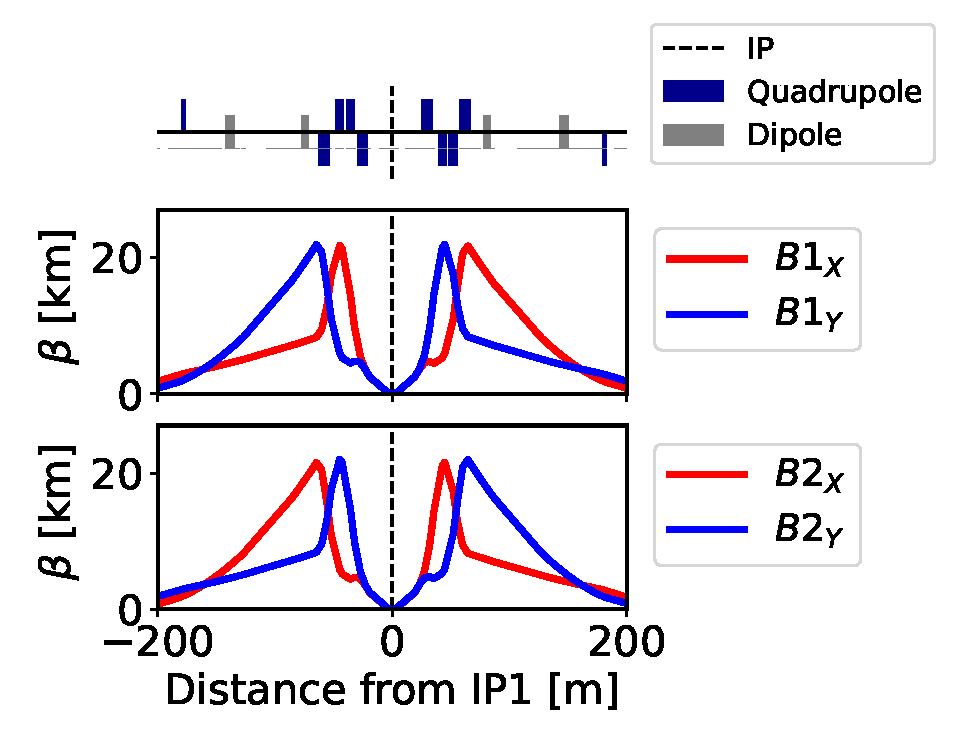
\includegraphics[height=60mm,trim=15 0 160 0, clip]{images/optics/plot.hllhc.round1515.xing_top.beta.IP1.pdf}
        \begin{tikzpicture}[every node/.style={inner sep=1pt,outer sep=0}]
            \node (image) at (current page.center) {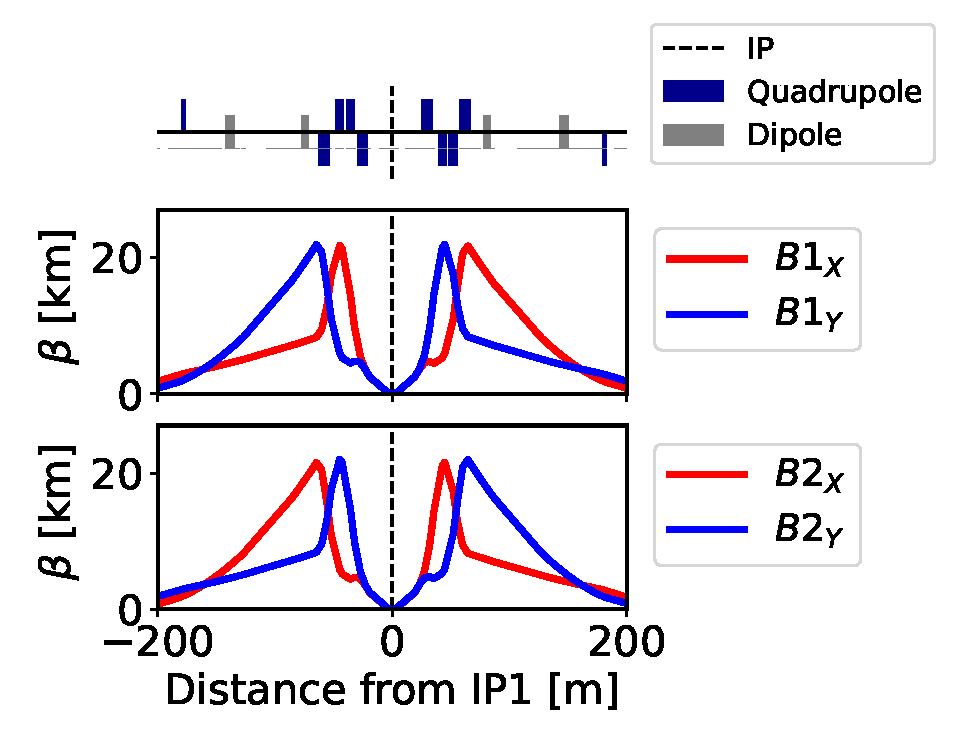
\includegraphics[height=60mm, trim=15 0 160 0, clip]{images/optics/plot.hllhc.round1515.xing_top.beta.IP1.pdf}};
            \begin{scope}[shift={(image.south west)},x={(image.south east)},y={(image.north west)}]
            \node (b1start) at (0.238, 0.454){};
            \node (b1)[right= 10pt of b1start] {\tiny Beam 1};
            \node (b1end)[right= 10pt of b1]{};
            \draw[-]  (b1start) -- (b1);
            \draw[->]  (b1) -- (b1end);
            \node (b2start) at (0.94, 0.454){};
            \node (b2)[left= 10pt of b2start] {\tiny Beam 2};
            \node (b2end)[left= 10pt of b2]{};
            \draw[-]  (b2start) -- (b2);
            \draw[->]  (b2) -- (b2end);
            \end{scope}
        \end{tikzpicture}
        \caption{$\beta^* = \qty{15}{cm}$ round optics}
        \label{fig:betaIP1HLLHCround}
    \end{subfigure}
    \begin{subfigure}[t]{0.35\textwidth}
        % 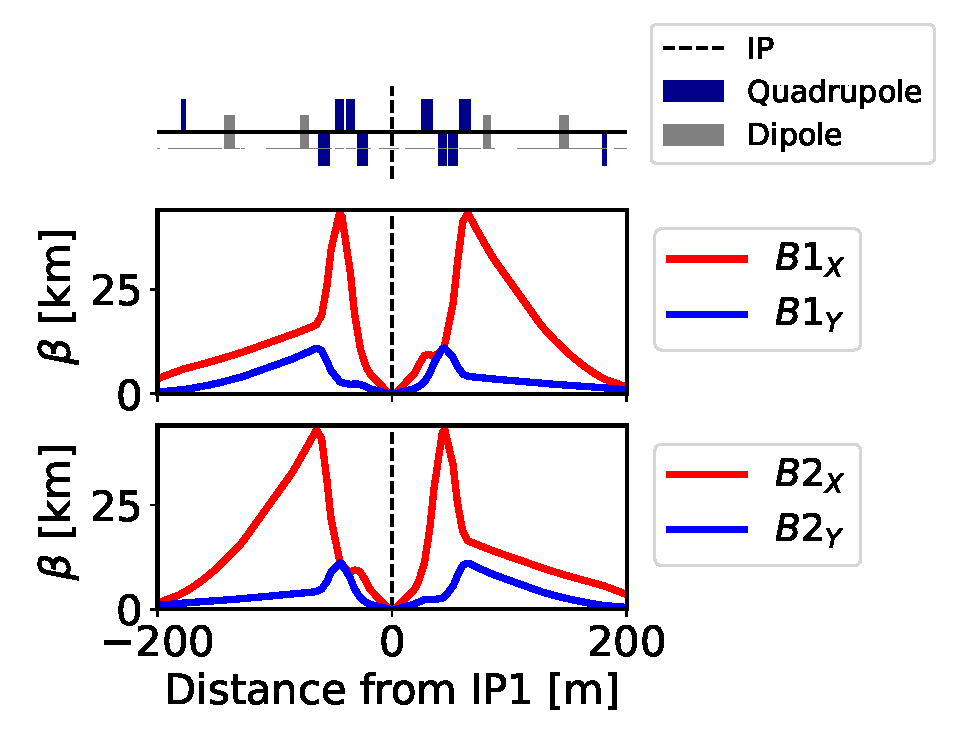
\includegraphics[height=60mm, trim=40 0 19 0, clip]{images/optics/plot.hllhc.flat07530.xing_top.beta.IP1.pdf}
        \begin{tikzpicture}[every node/.style={inner sep=1pt,outer sep=0}]
            \node (image) at (current page.center) {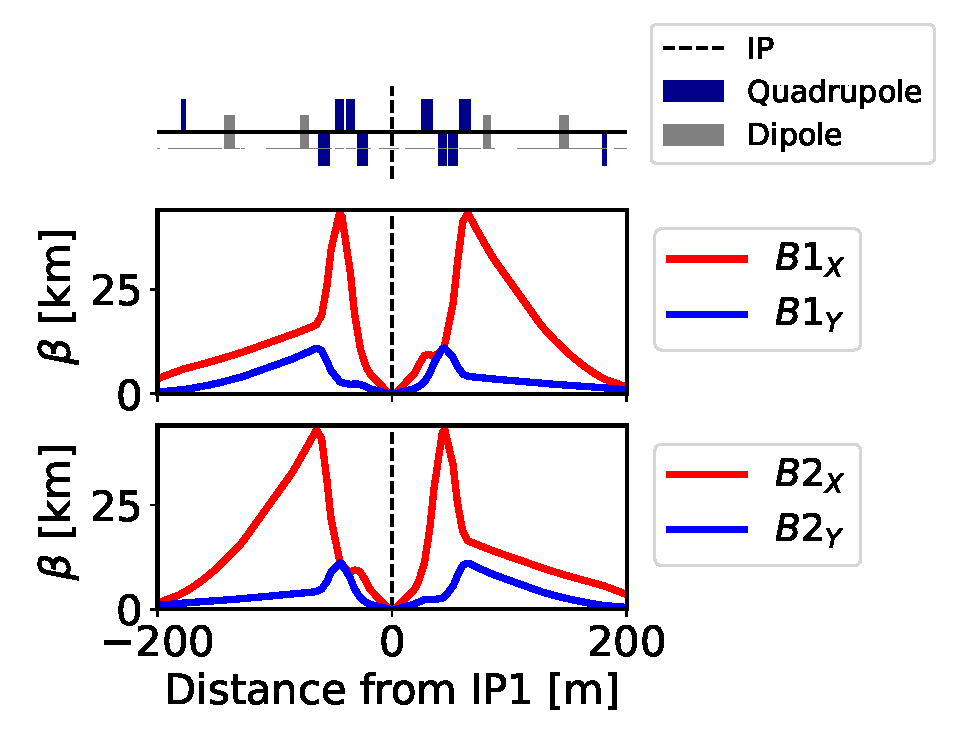
\includegraphics[height=60mm, trim=40 0 19 0, clip]{images/optics/plot.hllhc.flat07530.xing_top.beta.IP1.pdf}};
            \begin{scope}[shift={(image.south west)},x={(image.south east)},y={(image.north west)}]
            \node (b1start) at (0.107, 0.454){};
            \node (b1)[right= 10pt of b1start] {\tiny Beam 1};
            \node (b1end)[right= 10pt of b1]{};
            \draw[-]  (b1start) -- (b1);
            \draw[->]  (b1) -- (b1end);
            \node (b2start) at (0.62, 0.454){};
            \node (b2)[left= 10pt of b2start] {\tiny Beam 2};
            \node (b2end)[left= 10pt of b2]{};
            \draw[-]  (b2start) -- (b2);
            \draw[->]  (b2) -- (b2end);
            \end{scope}
        \end{tikzpicture}
        \caption{$\beta^*_{x/y} = \qty{7.5}{cm}/\qty{30}{cm}$ flat optics}
        \label{fig:betaIP1HLLHCflat}
    \end{subfigure}
	\caption{HL-LHC $\beta$-functions in the IR around IP1.}
	\label{fig:betaIP1HLLHC}
\end{figure}

In the original implementation of the algorithm in~\cite{BruningDynamicApertureStudies2004},
the optics of only one beam could be given and the algorithm was making use 
of the symmetries of the $\beta$-function in the IR
%
\begin{equation}
    \label{eq:betaSymmetriesRound}
    \begin{split}
        \beta_x^{\text{(B1)}}(s) &= \beta_y^{\text{(B2)}}(s) \\ 
        \beta_y^{\text{(B1)}}(s) &= \beta_x^{\text{(B2)}}(s) \;, 
    \end{split}
\end{equation}
%
which is true for round optics as shown in~\cref{fig:betaIP1HLLHCround}, to calculate a correction valid for both beams.
With this symmetry the effective RDT \cref{eq:effectiveRDT} simply switches the $\beta$ exponents between the beams, 
for which we will use the subscript {\scriptsize $jklm*$}: 
%
\begin{equation}
    \label{eq:effectiveRDT*}
    f^\text{IR (B1)}_{jklm*}  
    \;\; \overeq{\cref{eq:effectiveRDT}} \;\;
    \int\limits_\text{IR} 
    \ReOf{ 
     i^{l+m}
     \left(K_{n}(s) + iJ_{n}(s) \right) 
    }
        \beta^\text{(B1)}_x(s)^{\frac{l+m}{2}\;}
        \beta^\text{(B1)}_y(s)^{\frac{j+k}{2}} 
     e^{i \pi n \theta(s - s_\text{IP})}
    \mathrm{d}s 
    \;\; \overeq{\cref{eq:betaSymmetriesRound}} \;\;
    f^\text{IR (B2)}_{jklm}\; .
\end{equation}
%
As mentioned in the previous section, with the two correctors per field type (order and orientation),
we can perfectly correct two RDTs locally in the IR. 
When 
%
\begin{equation}
    j+k \equiv l+m \pmod{2} \;,
\end{equation}
%
i.e. both $f_{jklm}$ and $f_{lmjk}$ have the same orientation (skew or normal) RDTs, 
two RDTs per beam can be corrected, as $\left| i^{j+k} \right| = \left| i^{l+m} \right|$.
Therefore $\left| f^\text{IR}_{jklm*} \right| = \left| f^\text{IR}_{lmjk} \right|$ within the optics of the same beam
and we can choose $f^\text{IR}_{j'k'l'm'}  = f^\text{IR}_{lmjk} (= f^\text{IR}_{jklm*} \text{ or } -f^\text{IR}_{jklm*})$ in \cref{eq:linearEqSystemDouble}.
If, on the other hand, $j+k$ and $l+m$ are of different parity, only one RDT $f^\text{IR}_{jklm}$ per beam can be corrected, 
by targeting $f^\text{IR}_{jklm}$ and $f^\text{IR}_{j'k'l'm'} = f^\text{IR}_{jklm*}$ in the given optics.


\begin{important}
        \item[\color{BlackCat} Example] 
        To correct $b_4$, the two RDTs $f_{4000}$ and $f_{0040}$ can targeted,
        as both are normal octupole RDTs.
        $j+k$ and $l+m$ are both even ($i^{j+k} = i^{l+m}$), so correcting either one in one optics,
        will correct the respective other, in the other optics, e.g.
        %
        \begin{equation}
        \begin{split}
            f^\text{IR (B1)}_{4000} &= f^\text{IR (B1)}_{0040*} = f^\text{IR (B2)}_{0040} \;, \quad \text{and} \\
            f^\text{IR (B1)}_{0040} &=  f^\text{IR (B1)}_{4000*} = f^\text{IR (B2)}_{4000} \;.
        \end{split}
        \end{equation}
        %
        When correcting normal sextupole errors ($b_3$) on the other hand, we cannot target
        $f_{3000}$ and $f_{0030}$ as the latter targets a \textbf{skew} sextupole RDT.
        We can still target one RDT in each Beam, also by using just one optics 
        %
        \begin{equation}
        \begin{split}
            f^\text{IR (B1)}_{3000} &= f^\text{IR (B2)}_{3000*} \;, \quad \text{and} \\
            f^\text{IR (B1)}_{3000*} &=  f^\text{IR (B2)}_{3000} \;.
        \end{split}
        \end{equation}
        %
\end{important}

There are optics in which \cref{eq:betaSymmetriesRound} does not hold true anymore.
For example, in contrast to \textit{round} optics, 
in which the $\beta$-function  at the IP ($\beta^* = \beta(s_\text{IP})$) is equal for both transversal planes ($\beta^*_x = \beta^*_y$),
there exists also the \textit{flat} optics, for which $\beta^*_x \neq \beta^*_y$ 
(i.e. the beam shape is not round at the IP)~\cite{FartoukhAchromaticTelescopicSqueezing2013,FartoukhFlatTelescopicOptics2018}.
A realization of flat optics, forseen to be used in the HL-LHC, is shown in \cref{fig:betaIP1HLLHCflat}.

The straightforward way to not to rely on \cref{eq:betaSymmetriesRound}, 
is to use the optics for both beams in the correction and construct \cref{eq:linearEqSystemDouble} from both
%
\begin{equation}    
    \label{eq:linearEqSystemDoubleOptics}
        \begin{pmatrix}
            b_{jklm}^{(cl, \text{B1})} & b_{jklm}^{(cr, \text{B1})} \\
            b_{jklm}^{(cl, \text{B2})} & b_{jklm}^{(cr, \text{B2})}
        \end{pmatrix}
        \begin{pmatrix}
            K_{n}L_{cl} \\ 
            K_{n}L_{cr}
        \end{pmatrix}
        = - 
        \begin{pmatrix}
            I^{(\text{B1})}_{jklm} \\ 
            I^{(\text{B2})}_{jklm} 
        \end{pmatrix} 
        \; .
\end{equation}

\subsubsection{Feed-Down} % --------------------

The effect of feed-down occurs whenever a particle beam is passing off-center through a magnet, 
due to either a transverse misalignment of the magnet or an off-center closed orbit of the beam itself,
and results in the magnets exerting forces on the particles as lower-order magnets would, in addition
to their main component~\cite{WiedemannParticleAcceleratorPhysics2015}. 

Mathematically, feed-down can be understood by applying a first-order Taylor expansion 
to the Hamiltonian \cref{eq:hamiltonianTwissCoordinates} in the 
curvilinear (comoving) coordinate system and cartesian transversal coordinates
%
\begin{equation}
   \label{eq:hamiltonianComoving}
   h(x, y)
   = \qquad 
   -\ReOf{\sum_{n = 2}^\infty \left(K_n + iJ_n\right)\frac{\left(x + iy\right)^n}{n!}}
\end{equation}
%
for a beam centroid traversing the magnet at $\Delta x (s), \Delta y (s)$:
%
\begin{equation}
   \label{eq:hamiltonianFeeddownDerivation}
   \begin{split}
   h(x + \Delta x, y + \Delta y)
   &= \qquad 
   -\ReOf{\sum_{n = 2}^\infty \left(K_n + iJ_n\right)\frac{\left((x + \Delta x) +i (y + \Delta y)\right)^n}{n!}} \\
   &\overeq{\text{Taylor}} \qquad
    -\ReOf{
        \sum_{n = 2}^\infty (K_n + iJ_n)
        \frac{\sum\limits_{q=0}^{n} \frac{1}{q!} \frac{n!}{(n-q)!}(x+iy)^{n-q} (\Delta x + i \Delta y)^q}{n!}
    } \\
    &=\qquad
     -\ReOf{
         \sum_{n = 2}^\infty (K_n + iJ_n)
         \sum\limits_{q = 0}^{n} \frac{(x+iy)^{n-q} (\Delta x + i \Delta y)^q}{q!\, (n-q!)} 
      } \\
     &\myoverunder{\text{sort by } (x + iy)^n}{=}{n \mapsto n+q} \qquad
     - \ReOf{
        \sum_{n = 0}^\infty \sum_{q=\max(2-n, 0)}^{\infty} \frac{1}{q!\, n!}
        (K_{n+q} + iJ_{n+q}) (x + iy)^n (\Delta x + i \Delta y)^q 
     } \\
     &= \qquad
     - \ReOf{\sum_{n = 0}^\infty 
        \left( \sum_{q=\max(2-n, 0)}^{\infty} 
        (K_{n+q} + iJ_{n+q}) \frac{(\Delta x + i \Delta y)^q}{q!} \right)
        \frac{(x + iy)^n}{n!}
     }
   \end{split}
\end{equation}
%
For brevity $(s)$ is omitted, but $h, K_n, J_n, x, y$ and $\Delta x, \Delta y$ are all dependent on the longitudinal location.
From \cref{eq:hamiltonianComoving,eq:hamiltonianFeeddownDerivation} 
one can see that magnetic field strengths
of order $n \geq 2$ without offset are replaced by a sum depending on the 
higher order field strengths scaled by powers of the offset.
These higher order fields of $n+q$ therefore ``feed down'' to the field strengths of 
order $n$, showing the same effects on the beam as these lower orders would.
As seen in \cref{eq:hamiltonianFeeddownDerivation}, 
feed-down to field order $n \geq 2$ from fields up to $n + Q$ can be calculated by:
%
\begin{equation}
    \label{eq:feeddownOrderN}
    K_n + iJ_n \overset{\text{w/ feeddown}}{\rightarrow} \sum_{q = 0}^{Q} (K_{n+q} + iJ_{n+q}) \frac{(\Delta x + i \Delta y)^q}{q!}.
\end{equation}
%
Fields feed-down can also have an effect on the scalar field ($n = 0$) and dipole fields ($n = 1$).
As their structure does not follow the structure in \cref{eq:hamiltonianTwissCoordinates},
\cref{eq:feeddownOrderN} is not applicable.
In the context of RDTs $n$ is always larger than 2 and we can use \cref{eq:feeddownOrderN} 
in the definition of the effective RDT \cref{eq:effectiveRDT}
%
\begin{equation}
    \label{eq:effectiveRDTfeeddown}
    \small
    f^\text{IR}_{jklm} =  \int\limits_\text{IR} 
    \ReOf{    
     i^{l+m}
     \sum_{q = 0}^{\infty} 
     (K_{n+q}(s) + iJ_{n+q}(s)) \frac{(\Delta x(s) + i \Delta y(s))^q}{q!} 
    }
        \beta_x(s)^{\frac{j+k}{2}}
        \beta_y(s)^{\frac{l+m}{2}} 
     (-1)^{  n \theta(s - s_\text{IP})}
    \mathrm{d}s \; ,
\end{equation}
%
and can therefore easily include it when building the equation systems 
\cref{eq:linearEqSystemSingle}, \cref{eq:linearEqSystemDouble} or \cref{eq:linearEqSystemDoubleOptics}.

Not only can feed-down be used to calculate the influence of field errors of orders larger than $n$ on the RDTs of order $n$, 
i.e. by contributing to the integral $I_{jklm}$ on the right-hand side of the equation systems, 
but it can also be used to calculate the strengths of correctors of orders $n_\text{Corrector} > n$ 
to counteract the RDTs at order $n$ via feed-down, by including it on the left-hand side:
The matrix elements of the corrector coefficients in \cref{eq:BcomponentsDef} will then also contain the feed-down coefficient
%
\begin{equation}
    \label{eq:zpDefinition}
    z_{p} = \frac{\left( \Delta x + i\Delta y\right)^p}{p!} \, \,
\end{equation}
%
with $p$ being the order of feed-down from the corrector to the RDT, i.e. 
\begin{equation}
    \label{eq:DiffOrderCorrectorRDT}
    p = n_\text{Corrector} - n \, .
\end{equation}
%
As $z_p \in \mathbb{C}$, this makes the evaluation of the real part in \cref{eq:equationSum}, 
needed to split the equation system into two, separating the correctors (\cref{eq:linearEqSystemSingle}), 
less straightforward and more cases need to be considered.
Inserting
%
\begin{equation}
    \label{eq:KnJnWithZp}
    \begin{split}
        &\ReOf{    
        i^{l+m}
        (K_{n+p}L_w + iJ_{n+p}L_w) \frac{(\Delta xL_w + i \Delta yL_w)^q}{q!} 
        }
        \\
        \overeq{\cref{eq:zpDefinition}} \quad
        &\ReOf{    
        i^{l+m}
        (K_{n+p}L_w + iJ_{n+p}L_w) \cdot z_p 
        }
        \\
        =  \quad
        &\ReOf{    
        i^{l+m}
        (K_{n+p}L_w + iJ_{n+p}L_w) (\ReOf{z_p} + i\ImOf{z_p}) 
        }
        \\
        =  \quad
        &\ReOf{    
        i^{l+m} \left[
        (K_{n+p}L_w \cdot \ReOf{z_p} -J_{n+p}L_w \cdot \ImOf{z_p}) + i(K_{n+p}L_w \cdot \ImOf{z_p} + J_{n+p} \cdot \ReOf{z_p} )\right] 
        }
    \end{split}
\end{equation}
%
into \cref{eq:equationSum} yields the equation system
%
\begin{equation}
    \label{eq:linearEqSystemFeeddown}
    \begin{split}
    \footnotesize
    \begin{pmatrix}
        \ReOf{z_p} \cdot b_{jklm}^{(cl)} & 
        \ReOf{z_p} \cdot b_{jklm}^{(cr)} & 
        -\ImOf{z_p} \cdot b_{jklm}^{(cl)} &
        -\ImOf{z_p} \cdot b_{jklm}^{(cr)}
    \end{pmatrix}
    \begin{pmatrix}
        K_{n+p}L_{cl} \\ 
        K_{n+p}L_{cr} \\ 
        J_{n+p}L_{cl} \\ 
        J_{n+p}L_{cr}
    \end{pmatrix}
     &= -
     I_{jklm} \quad
    \text{for even } l+m, 
     \\
    \footnotesize
    \begin{pmatrix}
        i \,\ImOf{z_p} \cdot b_{jklm}^{(cl)} & 
        i \,\ImOf{z_p} \cdot b_{jklm}^{(cr)} & 
        i \,\ReOf{z_p} \cdot b_{jklm}^{(cl)} & 
        i \,\ReOf{z_p} \cdot b_{jklm}^{(cr)}
    \end{pmatrix}
    \begin{pmatrix}
        K_{n+p}L_{cl} \\ 
        K_{n+p}L_{cr} \\ 
        J_{n+p}L_{cl} \\
        J_{n+p}L_{cr}
    \end{pmatrix}
     &=  
     -I_{jklm} \quad
    \text{for odd } l+m \; .
    \end{split}
\end{equation}
%
In the case of $p = 0$, \cref{eq:linearEqSystemFeeddown} transforms back to \cref{eq:linearEqSystemSingle},
as $\ReOf{z_0} = 1$ and $\ImOf{z_0} = 0$. 
For simplicity, we can redefine $b_{jklm}$ to include the additional factors directly into the coefficients 
\begin{equation}
    \label{eq:coefficientWithFeeddown}
    b_{jklm,p} =
    \begin{cases}
      \phantom{-} \ReOf{z_p} \cdot b_{jklm}   \quad \text{if normal corrector and } l + m \text{ even}, \\
     \phantom{-} \ImOf{z_p} \cdot b_{jklm}    \quad \text{if normal corrector and } l + m \text{ odd}, \\    
      -\ImOf{z_p} \cdot b_{jklm}              \quad \text{if skew corrector and } l + m \text{ even}, \\    
       \phantom{-} \ReOf{z_p}  \cdot b_{jklm} \quad \text{if skew corrector and } l + m \text{ odd} 
    \end{cases}
\end{equation}
%
and take $z_p$ into account whenever $p>0$.

Including feed-down into the equation system also allows therefore to correct multiple orders of RDTs with the same correctors, 
as well as correcting RDTs with correctors of multiple orders.
\Cref{eq:linearEqSystemSingle} can hence not only be extended ``vertically'' by correcting for multiple beam optics (\cref{eq:linearEqSystemDoubleOptics})
 and different RDTs (\cref{eq:linearEqSystemDouble}) at the same time, 
but also ``horizontally'', by adding more correctors, e.g.
%
\begin{equation}    
    \label{eq:linearEqSystemDoubleCorrectors}
        \begin{pmatrix}
            b_{jklm}^{(cl)} & b_{jklm}^{(cr)} & b_{jklm,p}^{(cl)} & b_{jklm,p}^{(cr)} \\
            b_{j'k'l'm'}^{(cl)} & b_{j'k'l'm'}^{(cr)} & b_{j'k'l'm',p}^{(cl)} & b_{j'k'l'm',p}^{(cr)}
        \end{pmatrix}
        \begin{pmatrix}
            K_{n}L_{cl} \\ 
            K_{n}L_{cr} \\
            K_{n+p}L_{cl} \\ 
            K_{n+p}L_{cr}
        \end{pmatrix}
        = - 
        \begin{pmatrix}
            I_{jklm} \\ 
            I_{j'k'l'm'} 
        \end{pmatrix}
\end{equation}